
%%%%%%%%%%%%%%%%%%%%%%%%%%%%%%%%%%%
\chapter{Introduction}
%%%%%%%%%%%%%%%%%%%%%%%%%%%%%%%%%%%
	Over the past century humanity has become increasingly dependent on the 4th state of matter, plasma. Attaining a better understanding of plasma behaviour and interaction is critical to developing faster computer chips, creating new sources of energy, and expanding humanities influence amoung the stars. One important subset of plasma behaviour is how plasmas interact with solid objects such as dust particles, probes, and bodies traveling through space. These interactions can be very difficult to explore experimentally, and therefore must be modelled. 
	
A plasma's behaviour is heavily influenced by the collective electric and magnetic fields generated by the individual particles that comprise the plasma. This means that plasma behaviour is essentially a very large n-body problem, where for moderately dense plasmas n can be on the order of $10^{20}$. No computer currently in existence can store the information for $10^{20}$ particles, and calculating the interaction of every particle in the set with every other particle would be prohibitvely long. The solution to this problem is to model only a subset of the true number of particles. The modeled behaviour of these particles and their contributions to magnetic and electric fields can be used to statistically infer the behaviour of the rest of the plasma, essentially from first princeiples. This method is called particle-in-cell (PIC), and operates by moving particles on a potential grid and updating that potential with the new particle density at every timestep. The flow of a general PIC code is shown in figure \ref{fig:pic_flowchart}. The PIC method is a very robust and straightforward scheme for modeling plasma behaviour, and is used extensively to model plasmas in complicated systems.

\begin{figure}
\begin{center}

\includegraphics[width=4in]{introduction/not_finished.pdf}
\end{center}
\caption{Flow schematic for the PIC method. Need to make figure}
\label{fig:pic_flowchart}
\end{figure}


%%%%%%%%%%%%%%%%%%%%%%%%%%%%%%%%%%%% 
	\section{Motivation}
%%%%%%%%%%%%%%%%%%%%%%%%%%%%%%%%%%%%

	The PIC method is very good at modeling complicated plasma behaviour, however this method still relies on tracking a very large number of particles for good statistics. In order to achieve ``good'' statistics PIC codes employ millions to billions of particles, which means that these codes can require a very large amount of computation time for each timestep. Running millions of particles on a single processor for hundreds of timesteps is not really feasible, it simply takes too long to compute a solution. 
	
	One way to reduce the total run time of PIC codes is to parallelize them. Since PIC codes operate on the fact that the potential changes little over the course of a single timestep, each particle can be assumed to be independent of its neighbors. This leads to a situation that is trivially parallel. In theory a machine with a million processors could run every particle on a seperate processor. This is of course assuming that the majority of the computational complexity lies in moving the particles and that comunication between processors is very fast.  


%%%%%%%%%%%%%%%%%%%%%%%%%%%%%%%%%%%%
		\subsection{GPUs vs CPUs}
%%%%%%%%%%%%%%%%%%%%%%%%%%%%%%%%%%%%
	The ideal computing system for a particle in cell code should have a large number of relatively simple processors with very low communication costs. Traditional CPUs are just the oposite of this. CPUs tend to have 4-8 complicated processors that are very good at performing large operations on small sets of data, but very slow when it comes to communicating between multiple processors. CPUs are designed to be able to actively switch tasks on the fly. This makes them very good at simultaneously running web-browser, decoding a video, and playing a video game. However, this flexiblity requires a large number of cycles to switch between tasks, and a large amount of cache to store partially completed tasks.

Graphical processing units, or GPUs, forgoe the flexibility of CPUs in favor of more raw processing capability. Reducing the size of the cache and employing single instruction multiple data (SIMD) parallelism allows GPU manufactures to combine hundreds of processors on a single chip. In order to supply enough data to keep hundreds of processors GPUs also have a very large data channel between the processors and DRAM. All of these features are chosen to create a math processor that excels at tasks where each processor operates on data that is invisible to the other processors. These features give GPUs a significant raw floating point performance advantage over CPUs as seen in figure \ref{fig:gpu_vs_cpu}. 


\begin{figure}
\begin{center}
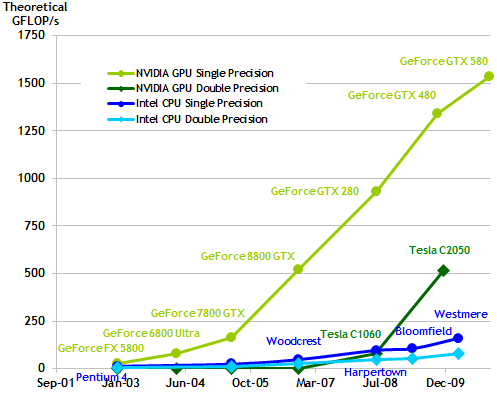
\includegraphics[width=4in]{introduction/gpu_vs_cpu.png}
\end{center}
\caption{Performance comparison of GPUs vs CPUs.}
\label{fig:gpu_vs_cpu}
\end{figure}

The hardware in GPUs is tailored to excel at performing tasks such as ray-tracing, which is very similar to particle moving. Therefore it is by no means unreasonable to conclude that GPUs can be very good PIC code processors. The advantages that GPUs have over CPUs for scientific computing include:

\begin{itemize}
	\item Higher performance per cost.
	\item Higher performance per watt.
	\item Easier to upgrade.
	\item GPUs still improving with Moore's law.
\end{itemize}

All of which are observed when comparing the CPU and GPU versions of the same PIC code. While these advantages are very promising there are also several disadvantages to GPU computing:

\begin{itemize}
	\item Increased code complexity.
	\item Smaller memory space.
	\item Smaller cache.
	\item Slow communication between CPU and GPU.
	\item Most developed GPU language is an extension of C.
	\item Algorithms can be very dependent on hardware configuration.
\end{itemize}

The key to developing efficient PIC algorithms that utilize GPUs lies in balancing the work between the two architectures. Some operations will be easier to implement on the CPU and be just as fast as the GPU while others will be significantly faster on the GPU. Partitioning the code between the different architectures begins to outline a very important aspect of parallel computing, multiple levels of parallelism.

%%%%%%%%%%%%%%%%%%%%%%%%%%%%%%%%%%%%
	\section{Multiple Levels of Parallelism}
%%%%%%%%%%%%%%%%%%%%%%%%%%%%%%%%%%%%
	Currently most parallelization is done by dividing up a task between a bunch of threads on different CPUs, and using an interface such as MPI to allow those threads to communicate. This network of threads has a master node, usually node 0, which orchestrates the communication between the other nodes. This is analgous to how a single CPU-GPU system operates. The CPU is the ``Master'' and serves as a communication hub for groups of execution threads on the GPU called thread blocks. Each thread block is itself a cluster of threads that can communicate through a memory space aptly named ``shared memory''.

\begin{figure}
\begin{center}
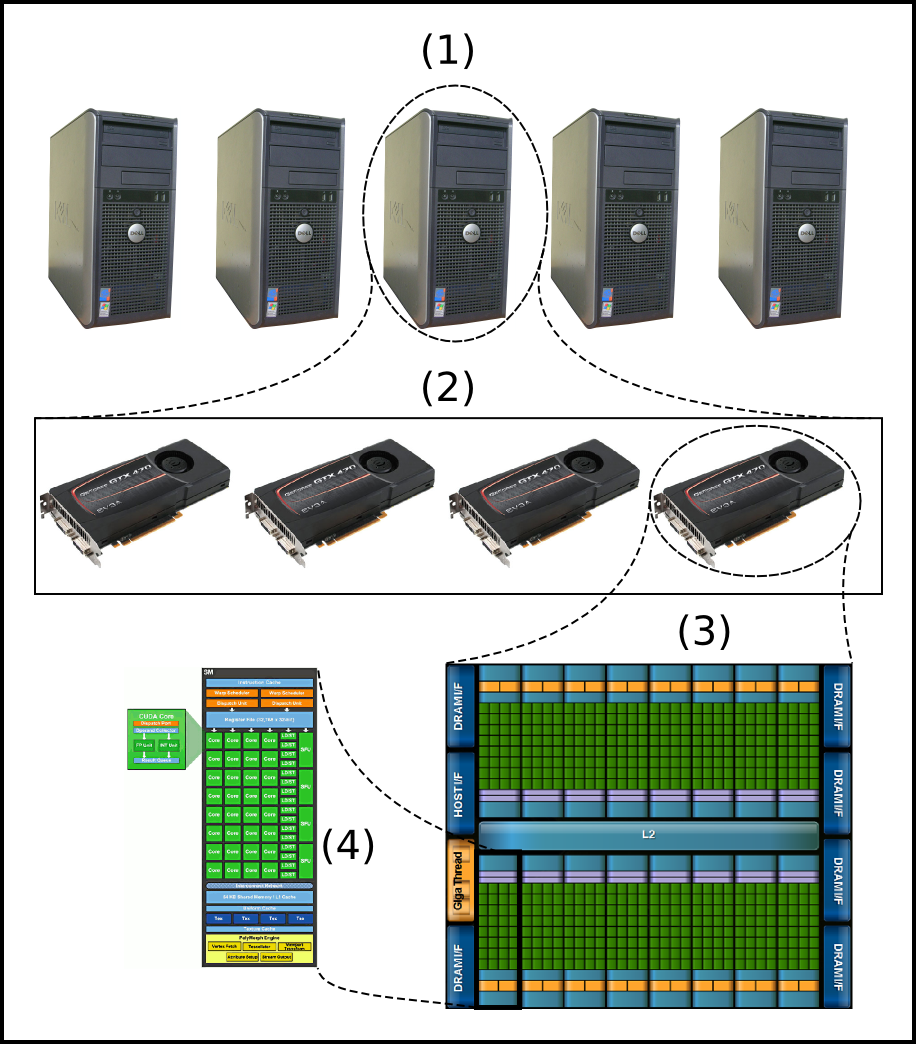
\includegraphics[width=5in]{introduction/multi_parallel.png}
\end{center}
\caption{Multiple levels of parallelism. (1) Cluster of systems communicating through a LAN. (2) Multiple GPUs per system communicating through system DRAM. (3) Multiple streaming multiprocessors per GPU execute thread-blocks and communicate through GPU global memory. (4) Multiple cuda cores per multiprocessor execute thread-warps and communicate through on chip shared memory. }
\label{fig:multiparallel}
\end{figure}

%%%%%%%%%%%%%%%%%%%%%%%%%%%%%%%%%%%%
		\subsection{Parallelization Opportunities in PIC Codes}
%%%%%%%%%%%%%%%%%%%%%%%%%%%%%%%%%%%%

\begin{figure}
\begin{center}

\includegraphics[width=4in]{introduction/not_finished.pdf}
\end{center}
\caption{Flow schematic for the PIC method with parallelizable steps highlighted. Need to make figure}
\label{fig:pic_flowchart_parallel}
\end{figure}

	
	\section{Overview of sceptic3D}











%%%%%%%%%%%%%%%%%%%%%%%%%%%%%%%%%%%%
	\chapter{Sceptic3D}
%%%%%%%%%%%%%%%%%%%%%%%%%%%%%%%%%%%%
Now that Sceptic3D is three dimensional hybrid PIC code specifically designed to solve the problem of ion flow past a negativley biased sphere in a uniform magnetic field. The current version of the code was derivied from the 2D/3v code SCEPTIC which was originally written by Hutchinson \cite{Hutchinson2002,Hutchinson2003,Hutchinson2005,Hutchinson2006}.



%%%%%%%%%%%%%%%%%%%%%%%%%%%%%%%%%%%%
		\section{Basic Code Structure}
%%%%%%%%%%%%%%%%%%%%%%%%%%%%%%%%%%%%
\begin{figure}
\begin{center}

\includegraphics[width=4in]{introduction/not_finished.pdf}
\end{center}
\caption{Flow schematic for the PIC method with sceptic subroutine names Need to make figure}
\label{fig:pic_flowchart_sceptic}
\end{figure}
		
		\subsection{Charge Assign Details}
		
		\subsection{Poisson Solve Details}
		
		\subsection{Particle Advancing Details}
		

		\section{CPU Code Profiling}

	\section{Overview of sceptic3Dgpu Goals}

		\subsection{Main Routines}

		\subsection{Supporting Routines}

		\subsection{Challenges to overcome}















